

\tikzset{every picture/.style={line width=0.75pt}} %set default line width to 0.75pt        

\begin{tikzpicture}[x=0.75pt,y=0.75pt,yscale=-1,xscale=1]
%uncomment if require: \path (0,464); %set diagram left start at 0, and has height of 464

%Image [id:dp23972146827135687] 
\draw (476.92,66.33) node  {
\includegraphics[width=22.13pt,height=22pt]{img/fig_one/verbal_instructions.jpg}};
%Image [id:dp27125135457739624] 
\draw (400.75,67.83) node  {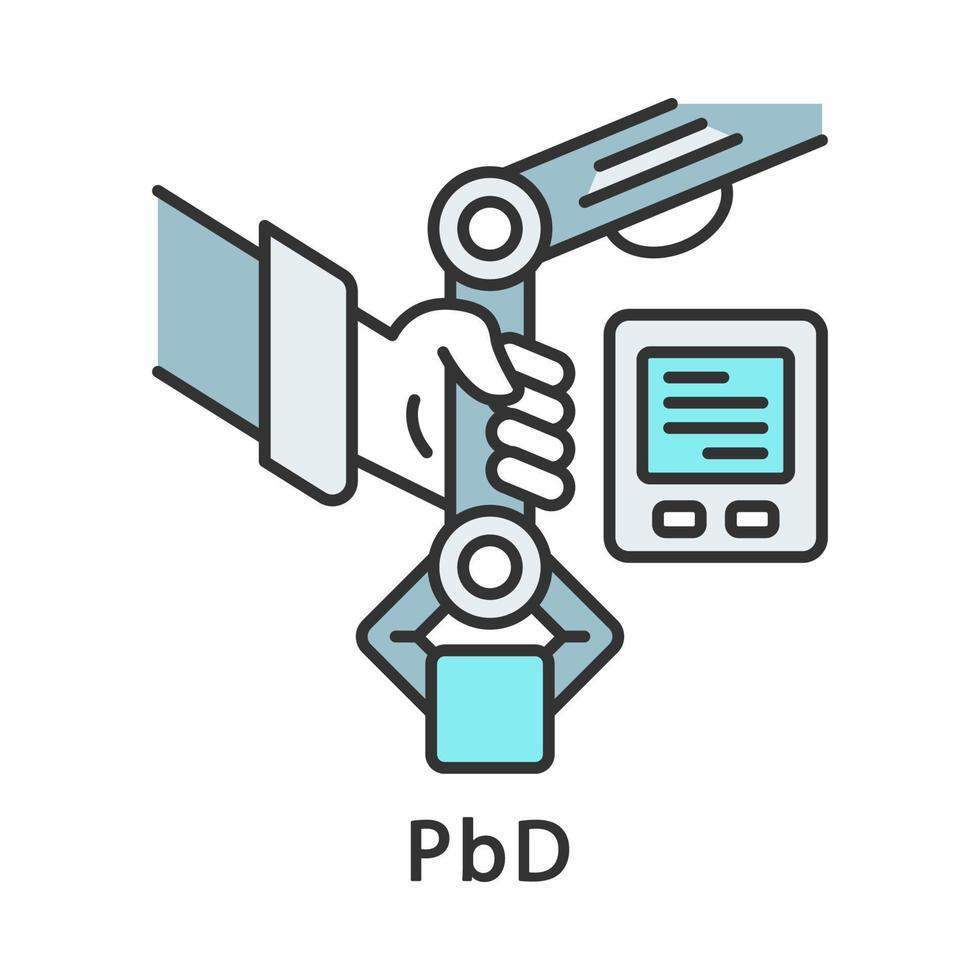
\includegraphics[width=24.13pt,height=21.75pt]{img/fig_one/demonstrations.jpg}};
%Shape: Rectangle [id:dp8290794414736217] 
\draw  [color={rgb, 255:red, 0; green, 0; blue, 0 }  ,draw opacity=0.7 ][fill={rgb, 255:red, 184; green, 233; blue, 134 }  ,fill opacity=0.25 ][line width=2.25]  (220.75,244.72) -- (587.5,244.72) -- (587.5,443.41) -- (220.75,443.41) -- cycle ;
%Shape: Rectangle [id:dp7997803732879841] 
\draw  [fill={rgb, 255:red, 74; green, 144; blue, 226 }  ,fill opacity=0.5 ] (234.76,274.72) -- (338.43,274.72) -- (338.43,316.59) -- (234.76,316.59) -- cycle ;
%Image [id:dp5448659080047329] 
\draw (262.81,290.08) node  {
\includegraphics[width=14.71pt,height=14.3pt]{img/fig_one/camera.png}};
%Shape: Ellipse [id:dp06339095907209769] 
\draw  [fill={rgb, 255:red, 74; green, 144; blue, 226 }  ,fill opacity=1 ] (318.98,286.49) .. controls (318.91,287.87) and (317.47,288.94) .. (315.76,288.88) .. controls (314.06,288.83) and (312.73,287.66) .. (312.8,286.28) .. controls (312.87,284.9) and (314.31,283.83) .. (316.02,283.89) .. controls (317.73,283.95) and (319.06,285.11) .. (318.98,286.49) -- cycle ;
%Shape: Ellipse [id:dp4388921464608323] 
\draw  [fill={rgb, 255:red, 74; green, 144; blue, 226 }  ,fill opacity=1 ] (318.75,279.29) .. controls (318.67,280.67) and (317.23,281.75) .. (315.52,281.69) .. controls (313.82,281.63) and (312.49,280.47) .. (312.56,279.09) .. controls (312.63,277.71) and (314.07,276.63) .. (315.78,276.69) .. controls (317.49,276.75) and (318.82,277.91) .. (318.75,279.29) -- cycle ;
%Shape: Ellipse [id:dp3507097342331216] 
\draw  [fill={rgb, 255:red, 74; green, 144; blue, 226 }  ,fill opacity=1 ] (319.06,293.91) .. controls (318.99,295.29) and (317.55,296.36) .. (315.84,296.3) .. controls (314.14,296.24) and (312.81,295.08) .. (312.88,293.7) .. controls (312.95,292.32) and (314.39,291.25) .. (316.1,291.3) .. controls (317.81,291.36) and (319.14,292.53) .. (319.06,293.91) -- cycle ;
%Shape: Ellipse [id:dp30210652412452677] 
\draw  [fill={rgb, 255:red, 74; green, 144; blue, 226 }  ,fill opacity=1 ] (318.96,301.54) .. controls (318.89,302.92) and (317.45,304) .. (315.74,303.94) .. controls (314.04,303.88) and (312.71,302.72) .. (312.78,301.34) .. controls (312.85,299.96) and (314.29,298.89) .. (316,298.94) .. controls (317.71,299) and (319.04,300.17) .. (318.96,301.54) -- cycle ;
%Shape: Ellipse [id:dp49480990786511814] 
\draw  [fill={rgb, 255:red, 74; green, 144; blue, 226 }  ,fill opacity=1 ] (305.56,283.05) .. controls (305.49,284.43) and (304.05,285.5) .. (302.34,285.44) .. controls (300.63,285.38) and (299.31,284.22) .. (299.38,282.84) .. controls (299.45,281.46) and (300.89,280.39) .. (302.6,280.45) .. controls (304.31,280.5) and (305.63,281.67) .. (305.56,283.05) -- cycle ;
%Shape: Ellipse [id:dp9963296119084144] 
\draw  [fill={rgb, 255:red, 74; green, 144; blue, 226 }  ,fill opacity=1 ] (305.52,290.27) .. controls (305.44,291.65) and (304,292.72) .. (302.29,292.66) .. controls (300.59,292.61) and (299.26,291.44) .. (299.33,290.06) .. controls (299.4,288.68) and (300.84,287.61) .. (302.55,287.67) .. controls (304.26,287.73) and (305.59,288.89) .. (305.52,290.27) -- cycle ;
%Shape: Ellipse [id:dp1365899025245182] 
\draw  [fill={rgb, 255:red, 74; green, 144; blue, 226 }  ,fill opacity=1 ] (305.49,297.87) .. controls (305.42,299.25) and (303.97,300.32) .. (302.27,300.26) .. controls (300.56,300.21) and (299.23,299.04) .. (299.3,297.66) .. controls (299.37,296.28) and (300.82,295.21) .. (302.52,295.27) .. controls (304.23,295.33) and (305.56,296.49) .. (305.49,297.87) -- cycle ;
%Shape: Ellipse [id:dp19251038300194467] 
\draw  [fill={rgb, 255:red, 74; green, 144; blue, 226 }  ,fill opacity=1 ] (294.77,290.27) .. controls (294.7,291.65) and (293.26,292.72) .. (291.55,292.66) .. controls (289.84,292.61) and (288.52,291.44) .. (288.59,290.06) .. controls (288.66,288.68) and (290.1,287.61) .. (291.81,287.67) .. controls (293.52,287.73) and (294.84,288.89) .. (294.77,290.27) -- cycle ;
%Straight Lines [id:da3317254092259251] 
\draw [fill={rgb, 255:red, 74; green, 144; blue, 226 }  ,fill opacity=1 ]   (312.78,301.34) -- (305.49,297.87) ;
%Straight Lines [id:da237977409467244] 
\draw [fill={rgb, 255:red, 74; green, 144; blue, 226 }  ,fill opacity=1 ]   (299.33,290.06) -- (294.77,290.27) ;
%Straight Lines [id:da9778691552033325] 
\draw [fill={rgb, 255:red, 74; green, 144; blue, 226 }  ,fill opacity=1 ]   (299.3,297.66) -- (294.77,290.27) ;
%Straight Lines [id:da5678771735843948] 
\draw [fill={rgb, 255:red, 74; green, 144; blue, 226 }  ,fill opacity=1 ]   (312.56,279.09) -- (305.56,283.05) ;
%Straight Lines [id:da563671631491371] 
\draw [fill={rgb, 255:red, 74; green, 144; blue, 226 }  ,fill opacity=1 ]   (312.56,279.09) -- (305.52,290.27) ;
%Straight Lines [id:da9988770219494821] 
\draw [fill={rgb, 255:red, 74; green, 144; blue, 226 }  ,fill opacity=1 ]   (312.56,279.09) -- (305.49,297.87) ;
%Straight Lines [id:da07427484805879225] 
\draw [fill={rgb, 255:red, 74; green, 144; blue, 226 }  ,fill opacity=1 ]   (312.8,286.28) -- (305.56,283.05) ;
%Straight Lines [id:da2932194957296641] 
\draw [fill={rgb, 255:red, 74; green, 144; blue, 226 }  ,fill opacity=1 ]   (312.8,286.28) -- (305.52,290.27) ;
%Straight Lines [id:da8113066636898383] 
\draw [fill={rgb, 255:red, 74; green, 144; blue, 226 }  ,fill opacity=1 ]   (312.8,286.28) -- (305.49,297.87) ;
%Straight Lines [id:da9649617409085037] 
\draw [fill={rgb, 255:red, 74; green, 144; blue, 226 }  ,fill opacity=1 ]   (312.88,293.7) -- (305.56,283.05) ;
%Straight Lines [id:da5233309778643113] 
\draw [fill={rgb, 255:red, 74; green, 144; blue, 226 }  ,fill opacity=1 ]   (312.88,293.7) -- (305.52,290.27) ;
%Straight Lines [id:da7738697746324189] 
\draw [fill={rgb, 255:red, 74; green, 144; blue, 226 }  ,fill opacity=1 ]   (312.88,293.7) -- (305.49,297.87) ;
%Straight Lines [id:da36188086063509384] 
\draw [fill={rgb, 255:red, 74; green, 144; blue, 226 }  ,fill opacity=1 ]   (312.78,301.34) -- (305.56,283.05) ;
%Straight Lines [id:da7668959348691485] 
\draw [fill={rgb, 255:red, 74; green, 144; blue, 226 }  ,fill opacity=1 ]   (312.78,301.34) -- (305.52,290.27) ;
%Straight Lines [id:da7590955635235813] 
\draw [fill={rgb, 255:red, 74; green, 144; blue, 226 }  ,fill opacity=1 ]   (299.38,282.84) -- (294.77,290.27) ;

%Shape: Rectangle [id:dp1797395110084451] 
\draw  [fill={rgb, 255:red, 122; green, 238; blue, 1 }  ,fill opacity=0.25 ] (27.79,159.48) -- (142.25,159.48) -- (142.25,204.91) -- (27.79,204.91) -- cycle ;
%Straight Lines [id:da08104897723298254] 
\draw [color={rgb, 255:red, 65; green, 117; blue, 5 }  ,draw opacity=1 ][line width=1.5]    (390.4,128) -- (390.75,156.2) ;
\draw [shift={(390.8,160.2)}, rotate = 269.29] [fill={rgb, 255:red, 65; green, 117; blue, 5 }  ,fill opacity=1 ][line width=0.08]  [draw opacity=0] (9.29,-4.46) -- (0,0) -- (9.29,4.46) -- cycle    ;
%Straight Lines [id:da761803787109346] 
\draw [line width=2.25]    (355.5,21.87) -- (492.9,21.27) -- (492.83,31) ;
\draw [shift={(492.79,36)}, rotate = 270.42] [fill={rgb, 255:red, 0; green, 0; blue, 0 }  ][line width=0.08]  [draw opacity=0] (11.43,-5.49) -- (0,0) -- (11.43,5.49) -- cycle    ;
%Straight Lines [id:da6542780963806372] 
\draw [line width=0.75]    (370.8,127.2) -- (634.5,127.33) ;
%Image [id:dp21737842353330383] 
\draw (541.48,380.58) node  {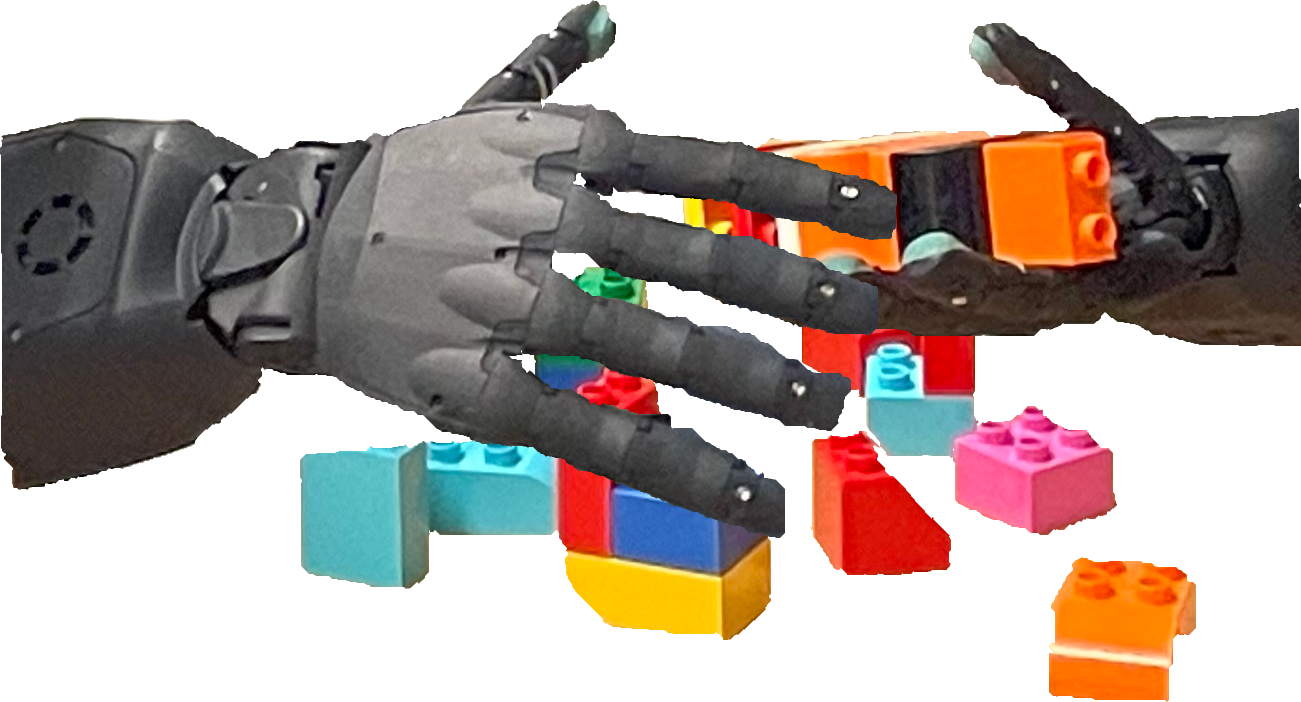
\includegraphics[width=44.63pt,height=39.5pt]{img/fig_one/real_world.png}};
%Shape: Rectangle [id:dp8123618146902207] 
\draw   (501.4,352.58) -- (580.57,352.58) -- (580.57,422.92) -- (501.4,422.92) -- cycle ;

%Image [id:dp6051084091861239] 
\draw (541.4,309.25) node  {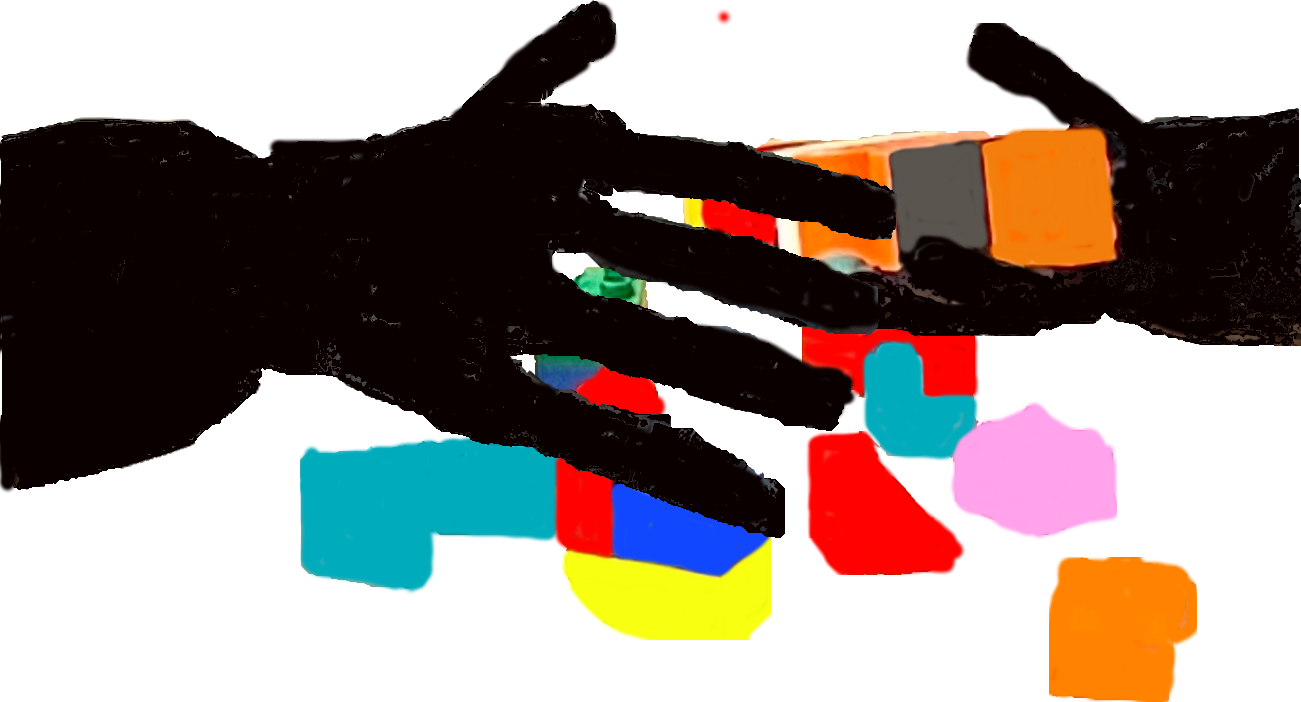
\includegraphics[width=46.25pt,height=39.5pt]{img/fig_one/simulation.png}};
%Shape: Rectangle [id:dp9413655175611488] 
\draw   (501.73,280.58) -- (580.9,280.58) -- (580.9,350.92) -- (501.73,350.92) -- cycle ;

%Shape: Rectangle [id:dp775617935041862] 
\draw  [fill={rgb, 255:red, 144; green, 19; blue, 254 }  ,fill opacity=0.5 ] (234.89,330.38) -- (338.56,330.38) -- (338.56,372.26) -- (234.89,372.26) -- cycle ;
%Shape: Ellipse [id:dp8684429829270282] 
\draw  [fill={rgb, 255:red, 144; green, 19; blue, 254 }  ,fill opacity=1 ] (324.12,341.16) .. controls (324.05,342.54) and (322.6,343.61) .. (320.9,343.55) .. controls (319.19,343.49) and (317.86,342.33) .. (317.93,340.95) .. controls (318,339.57) and (319.45,338.5) .. (321.15,338.55) .. controls (322.86,338.61) and (324.19,339.78) .. (324.12,341.16) -- cycle ;
%Shape: Ellipse [id:dp15790921758301146] 
\draw  [fill={rgb, 255:red, 144; green, 19; blue, 254 }  ,fill opacity=1 ] (323.88,333.96) .. controls (323.81,335.34) and (322.37,336.41) .. (320.66,336.35) .. controls (318.95,336.3) and (317.62,335.13) .. (317.69,333.75) .. controls (317.77,332.37) and (319.21,331.3) .. (320.91,331.36) .. controls (322.62,331.42) and (323.95,332.58) .. (323.88,333.96) -- cycle ;
%Shape: Ellipse [id:dp039266906086042774] 
\draw  [fill={rgb, 255:red, 144; green, 19; blue, 254 }  ,fill opacity=1 ] (324.2,348.57) .. controls (324.13,349.95) and (322.68,351.02) .. (320.98,350.97) .. controls (319.27,350.91) and (317.94,349.74) .. (318.01,348.36) .. controls (318.08,346.98) and (319.53,345.91) .. (321.23,345.97) .. controls (322.94,346.03) and (324.27,347.19) .. (324.2,348.57) -- cycle ;
%Shape: Ellipse [id:dp42148761281423] 
\draw  [fill={rgb, 255:red, 144; green, 19; blue, 254 }  ,fill opacity=1 ] (324.1,356.21) .. controls (324.03,357.59) and (322.58,358.66) .. (320.88,358.61) .. controls (319.17,358.55) and (317.84,357.38) .. (317.91,356) .. controls (317.98,354.62) and (319.43,353.55) .. (321.13,353.61) .. controls (322.84,353.67) and (324.17,354.83) .. (324.1,356.21) -- cycle ;
%Shape: Ellipse [id:dp18311865216474021] 
\draw  [fill={rgb, 255:red, 144; green, 19; blue, 254 }  ,fill opacity=1 ] (310.7,337.71) .. controls (310.63,339.09) and (309.18,340.17) .. (307.48,340.11) .. controls (305.77,340.05) and (304.44,338.89) .. (304.51,337.51) .. controls (304.58,336.13) and (306.02,335.05) .. (307.73,335.11) .. controls (309.44,335.17) and (310.77,336.33) .. (310.7,337.71) -- cycle ;
%Shape: Ellipse [id:dp6593766439126378] 
\draw  [fill={rgb, 255:red, 144; green, 19; blue, 254 }  ,fill opacity=1 ] (310.65,344.94) .. controls (310.58,346.32) and (309.14,347.39) .. (307.43,347.33) .. controls (305.72,347.27) and (304.39,346.11) .. (304.46,344.73) .. controls (304.54,343.35) and (305.98,342.28) .. (307.69,342.34) .. controls (309.39,342.39) and (310.72,343.56) .. (310.65,344.94) -- cycle ;
%Shape: Ellipse [id:dp0646060392964698] 
\draw  [fill={rgb, 255:red, 144; green, 19; blue, 254 }  ,fill opacity=1 ] (310.62,352.54) .. controls (310.55,353.92) and (309.11,354.99) .. (307.4,354.93) .. controls (305.69,354.87) and (304.37,353.71) .. (304.44,352.33) .. controls (304.51,350.95) and (305.95,349.88) .. (307.66,349.94) .. controls (309.37,349.99) and (310.69,351.16) .. (310.62,352.54) -- cycle ;
%Shape: Ellipse [id:dp344241482035639] 
\draw  [fill={rgb, 255:red, 144; green, 19; blue, 254 }  ,fill opacity=1 ] (299.91,344.94) .. controls (299.83,346.32) and (298.39,347.39) .. (296.68,347.33) .. controls (294.98,347.27) and (293.65,346.11) .. (293.72,344.73) .. controls (293.79,343.35) and (295.23,342.28) .. (296.94,342.34) .. controls (298.65,342.39) and (299.98,343.56) .. (299.91,344.94) -- cycle ;
%Straight Lines [id:da053308123146677766] 
\draw [fill={rgb, 255:red, 144; green, 19; blue, 254 }  ,fill opacity=1 ]   (317.91,356) -- (310.62,352.54) ;
%Straight Lines [id:da9308169262959871] 
\draw [fill={rgb, 255:red, 144; green, 19; blue, 254 }  ,fill opacity=1 ]   (304.46,344.73) -- (299.9,344.94) ;
%Straight Lines [id:da9623112310201266] 
\draw [fill={rgb, 255:red, 144; green, 19; blue, 254 }  ,fill opacity=1 ]   (304.44,352.33) -- (299.9,344.94) ;
%Straight Lines [id:da3713083923100239] 
\draw [fill={rgb, 255:red, 144; green, 19; blue, 254 }  ,fill opacity=1 ]   (317.69,333.75) -- (310.7,337.71) ;
%Straight Lines [id:da7378833559687352] 
\draw [fill={rgb, 255:red, 144; green, 19; blue, 254 }  ,fill opacity=1 ]   (317.69,333.75) -- (310.65,344.94) ;
%Straight Lines [id:da8085072888202742] 
\draw [fill={rgb, 255:red, 144; green, 19; blue, 254 }  ,fill opacity=1 ]   (317.69,333.75) -- (310.62,352.54) ;
%Straight Lines [id:da33461816065187067] 
\draw [fill={rgb, 255:red, 144; green, 19; blue, 254 }  ,fill opacity=1 ]   (317.93,340.95) -- (310.7,337.71) ;
%Straight Lines [id:da2436871845077183] 
\draw [fill={rgb, 255:red, 144; green, 19; blue, 254 }  ,fill opacity=1 ]   (317.93,340.95) -- (310.65,344.94) ;
%Straight Lines [id:da3325352556660157] 
\draw [fill={rgb, 255:red, 144; green, 19; blue, 254 }  ,fill opacity=1 ]   (317.93,340.95) -- (310.62,352.54) ;
%Straight Lines [id:da8548719045537613] 
\draw [fill={rgb, 255:red, 144; green, 19; blue, 254 }  ,fill opacity=1 ]   (318.01,348.36) -- (310.7,337.71) ;
%Straight Lines [id:da30441622065300544] 
\draw [fill={rgb, 255:red, 144; green, 19; blue, 254 }  ,fill opacity=1 ]   (318.01,348.36) -- (310.65,344.94) ;
%Straight Lines [id:da2551211262938834] 
\draw [fill={rgb, 255:red, 144; green, 19; blue, 254 }  ,fill opacity=1 ]   (318.01,348.36) -- (310.62,352.54) ;
%Straight Lines [id:da10799980447120472] 
\draw [fill={rgb, 255:red, 144; green, 19; blue, 254 }  ,fill opacity=1 ]   (317.91,356) -- (310.7,337.71) ;
%Straight Lines [id:da4719731970897004] 
\draw [fill={rgb, 255:red, 144; green, 19; blue, 254 }  ,fill opacity=1 ]   (317.91,356) -- (310.65,344.94) ;
%Straight Lines [id:da34564050701371696] 
\draw [fill={rgb, 255:red, 144; green, 19; blue, 254 }  ,fill opacity=1 ]   (304.51,337.51) -- (299.9,344.94) ;

%Image [id:dp48575653498321447] 
\draw (265.9,344.6) node  {
\includegraphics[width=16pt,height=14.5pt]{img/fig_one/world.png}};
%Shape: Rectangle [id:dp523016715222428] 
\draw   (498.6,276.8) -- (583.4,276.8) -- (583.4,425.2) -- (498.6,425.2) -- cycle ;
%Shape: Rectangle [id:dp15543160037895853] 
\draw  [fill={rgb, 255:red, 248; green, 231; blue, 28 }  ,fill opacity=0.25 ] (461.33,161.38) -- (538.67,161.38) -- (538.67,197.33) -- (461.33,197.33) -- cycle ;
%Shape: Rectangle [id:dp6451316862470362] 
\draw  [fill={rgb, 255:red, 248; green, 231; blue, 28 }  ,fill opacity=0.25 ] (373.67,161.22) -- (441.67,161.22) -- (441.67,197.67) -- (373.67,197.67) -- cycle ;
%Straight Lines [id:da29622460057420175] 
\draw [color={rgb, 255:red, 74; green, 144; blue, 226 }  ,draw opacity=1 ][line width=1.5]    (488.4,128) -- (488.05,156) ;
\draw [shift={(488,160)}, rotate = 270.72] [fill={rgb, 255:red, 74; green, 144; blue, 226 }  ,fill opacity=1 ][line width=0.08]  [draw opacity=0] (9.29,-4.46) -- (0,0) -- (9.29,4.46) -- cycle    ;
%Straight Lines [id:da37767414194756854] 
\draw [color={rgb, 255:red, 144; green, 19; blue, 254 }  ,draw opacity=1 ][line width=1.5]    (510.83,128) -- (510.63,156) ;
\draw [shift={(510.6,160)}, rotate = 270.42] [fill={rgb, 255:red, 144; green, 19; blue, 254 }  ,fill opacity=1 ][line width=0.08]  [draw opacity=0] (9.29,-4.46) -- (0,0) -- (9.29,4.46) -- cycle    ;
%Straight Lines [id:da1897982660355162] 
\draw [color={rgb, 255:red, 65; green, 117; blue, 5 }  ,draw opacity=1 ][line width=1.5]    (38.63,158.25) -- (38.4,41) -- (199.5,40.35) ;
\draw [shift={(203.5,40.33)}, rotate = 179.77] [fill={rgb, 255:red, 65; green, 117; blue, 5 }  ,fill opacity=1 ][line width=0.08]  [draw opacity=0] (9.29,-4.46) -- (0,0) -- (9.29,4.46) -- cycle    ;
%Straight Lines [id:da5174032935682547] 
\draw [color={rgb, 255:red, 74; green, 144; blue, 226 }  ,draw opacity=1 ][line width=1.5]    (70.63,158.25) -- (71.45,64.2) -- (198.75,64.01) ;
\draw [shift={(202.75,64)}, rotate = 179.91] [fill={rgb, 255:red, 74; green, 144; blue, 226 }  ,fill opacity=1 ][line width=0.08]  [draw opacity=0] (9.29,-4.46) -- (0,0) -- (9.29,4.46) -- cycle    ;
%Straight Lines [id:da4379641175048674] 
\draw [color={rgb, 255:red, 144; green, 19; blue, 254 }  ,draw opacity=1 ][line width=1.5]    (97.63,158.5) -- (98.6,87.2) -- (198.63,87.25) ;
\draw [shift={(202.63,87.25)}, rotate = 180.03] [fill={rgb, 255:red, 144; green, 19; blue, 254 }  ,fill opacity=1 ][line width=0.08]  [draw opacity=0] (9.29,-4.46) -- (0,0) -- (9.29,4.46) -- cycle    ;
%Straight Lines [id:da7113187730392087] 
\draw [color={rgb, 255:red, 65; green, 117; blue, 5 }  ,draw opacity=0.5 ][line width=1.5]    (390.65,199.25) -- (390.69,207.93) -- (390.73,215.25) ;
\draw [shift={(390.75,219.25)}, rotate = 269.71] [fill={rgb, 255:red, 65; green, 117; blue, 5 }  ,fill opacity=0.5 ][line width=0.08]  [draw opacity=0] (9.29,-4.46) -- (0,0) -- (9.29,4.46) -- cycle    ;
%Shape: Rectangle [id:dp975711624614093] 
\draw  [color={rgb, 255:red, 0; green, 0; blue, 0 }  ,draw opacity=0.7 ][line width=1.5]  (103.75,279.55) -- (160.5,279.55) -- (160.5,444.5) -- (103.75,444.5) -- cycle ;
%Curve Right Arrow [id:dp755472264545883] 
\draw  [color={rgb, 255:red, 0; green, 0; blue, 0 }  ,draw opacity=0.3 ][fill={rgb, 255:red, 245; green, 166; blue, 35 }  ,fill opacity=0.5 ] (249,216.29) .. controls (249,206.93) and (230.73,199.33) .. (208.19,199.33) -- (208.19,187.09) .. controls (230.73,187.09) and (249,194.68) .. (249,204.05) ;\draw  [color={rgb, 255:red, 0; green, 0; blue, 0 }  ,draw opacity=0.3 ][fill={rgb, 255:red, 245; green, 166; blue, 35 }  ,fill opacity=0.5 ] (249,204.05) .. controls (249,211) and (238.93,216.98) .. (224.51,219.6) -- (224.51,215.52) -- (208.19,227.13) -- (224.51,235.92) -- (224.51,231.84) .. controls (238.93,229.22) and (249,223.25) .. (249,216.29)(249,204.05) -- (249,216.29) ;
%Curve Right Arrow [id:dp4614496757181181] 
\draw  [color={rgb, 255:red, 0; green, 0; blue, 0 }  ,draw opacity=0.3 ][fill={rgb, 255:red, 245; green, 166; blue, 35 }  ,fill opacity=0.5 ] (143.87,204.54) .. controls (143.87,213.91) and (162.14,221.5) .. (184.68,221.5) -- (184.68,233.74) .. controls (162.14,233.74) and (143.87,226.15) .. (143.87,216.78) ;\draw  [color={rgb, 255:red, 0; green, 0; blue, 0 }  ,draw opacity=0.3 ][fill={rgb, 255:red, 245; green, 166; blue, 35 }  ,fill opacity=0.5 ] (143.87,216.78) .. controls (143.87,209.83) and (153.94,203.85) .. (168.35,201.24) -- (168.35,205.32) -- (184.68,193.7) -- (168.35,184.91) -- (168.35,188.99) .. controls (153.94,191.61) and (143.87,197.59) .. (143.87,204.54)(143.87,216.78) -- (143.87,204.54) ;
%Shape: Rectangle [id:dp05918868424043677] 
\draw  [fill={rgb, 255:red, 248; green, 231; blue, 28 }  ,fill opacity=0.25 ] (557.17,161.38) -- (632.84,161.38) -- (632.84,197.33) -- (557.17,197.33) -- cycle ;
%Straight Lines [id:da5816109512295018] 
\draw [color={rgb, 255:red, 65; green, 117; blue, 5 }  ,draw opacity=1 ][line width=1.5]    (465.83,128) -- (465.8,156.2) ;
\draw [shift={(465.8,160.2)}, rotate = 270.06] [fill={rgb, 255:red, 65; green, 117; blue, 5 }  ,fill opacity=1 ][line width=0.08]  [draw opacity=0] (9.29,-4.46) -- (0,0) -- (9.29,4.46) -- cycle    ;
%Straight Lines [id:da3520850646821835] 
\draw [color={rgb, 255:red, 74; green, 144; blue, 226 }  ,draw opacity=1 ][line width=1.5]    (584.4,128) -- (584.05,156) ;
\draw [shift={(584,160)}, rotate = 270.72] [fill={rgb, 255:red, 74; green, 144; blue, 226 }  ,fill opacity=1 ][line width=0.08]  [draw opacity=0] (9.29,-4.46) -- (0,0) -- (9.29,4.46) -- cycle    ;
%Straight Lines [id:da32522639906583095] 
\draw [color={rgb, 255:red, 144; green, 19; blue, 254 }  ,draw opacity=1 ][line width=1.5]    (604.83,128) -- (604.63,156) ;
\draw [shift={(604.6,160)}, rotate = 270.42] [fill={rgb, 255:red, 144; green, 19; blue, 254 }  ,fill opacity=1 ][line width=0.08]  [draw opacity=0] (9.29,-4.46) -- (0,0) -- (9.29,4.46) -- cycle    ;
%Straight Lines [id:da7763193691001422] 
\draw [color={rgb, 255:red, 65; green, 117; blue, 5 }  ,draw opacity=1 ][line width=1.5]    (563.4,128) -- (563.75,156.2) ;
\draw [shift={(563.8,160.2)}, rotate = 269.29] [fill={rgb, 255:red, 65; green, 117; blue, 5 }  ,fill opacity=1 ][line width=0.08]  [draw opacity=0] (9.29,-4.46) -- (0,0) -- (9.29,4.46) -- cycle    ;
%Straight Lines [id:da3592857671981601] 
\draw [color={rgb, 255:red, 74; green, 144; blue, 226 }  ,draw opacity=0.5 ][line width=1.5]    (488.4,198) -- (488.08,215.07) ;
\draw [shift={(488,219.07)}, rotate = 271.09] [fill={rgb, 255:red, 74; green, 144; blue, 226 }  ,fill opacity=0.5 ][line width=0.08]  [draw opacity=0] (9.29,-4.46) -- (0,0) -- (9.29,4.46) -- cycle    ;
%Straight Lines [id:da5700192205968191] 
\draw [color={rgb, 255:red, 144; green, 19; blue, 254 }  ,draw opacity=0.5 ][line width=1.5]    (510.83,198) -- (510.64,215.07) ;
\draw [shift={(510.6,219.07)}, rotate = 270.63] [fill={rgb, 255:red, 144; green, 19; blue, 254 }  ,fill opacity=0.5 ][line width=0.08]  [draw opacity=0] (9.29,-4.46) -- (0,0) -- (9.29,4.46) -- cycle    ;
%Straight Lines [id:da628597817308811] 
\draw [color={rgb, 255:red, 65; green, 117; blue, 5 }  ,draw opacity=0.5 ][line width=1.5]    (465.83,198.67) -- (465.81,215.2) ;
\draw [shift={(465.8,219.2)}, rotate = 270.09] [fill={rgb, 255:red, 65; green, 117; blue, 5 }  ,fill opacity=0.5 ][line width=0.08]  [draw opacity=0] (9.29,-4.46) -- (0,0) -- (9.29,4.46) -- cycle    ;
%Straight Lines [id:da749451065817661] 
\draw [line width=0.75]    (305.8,244.2) -- (584.83,244) ;
%Straight Lines [id:da7350927289371181] 
\draw [color={rgb, 255:red, 74; green, 144; blue, 226 }  ,draw opacity=0.5 ][line width=1.5]    (584.4,198.33) -- (584.08,215.07) ;
\draw [shift={(584,219.07)}, rotate = 271.11] [fill={rgb, 255:red, 74; green, 144; blue, 226 }  ,fill opacity=0.5 ][line width=0.08]  [draw opacity=0] (9.29,-4.46) -- (0,0) -- (9.29,4.46) -- cycle    ;
%Straight Lines [id:da6732686021791007] 
\draw [color={rgb, 255:red, 144; green, 19; blue, 254 }  ,draw opacity=0.5 ][line width=1.5]    (603.83,198.33) -- (603.65,215.07) ;
\draw [shift={(603.6,219.07)}, rotate = 270.64] [fill={rgb, 255:red, 144; green, 19; blue, 254 }  ,fill opacity=0.5 ][line width=0.08]  [draw opacity=0] (9.29,-4.46) -- (0,0) -- (9.29,4.46) -- cycle    ;
%Straight Lines [id:da6752198515132564] 
\draw [color={rgb, 255:red, 65; green, 117; blue, 5 }  ,draw opacity=0.5 ][line width=1.5]    (563.4,198.33) -- (563.72,215.2) ;
\draw [shift={(563.8,219.2)}, rotate = 268.9] [fill={rgb, 255:red, 65; green, 117; blue, 5 }  ,fill opacity=0.5 ][line width=0.08]  [draw opacity=0] (9.29,-4.46) -- (0,0) -- (9.29,4.46) -- cycle    ;
%Shape: Rectangle [id:dp2692455293865468] 
\draw  [fill={rgb, 255:red, 208; green, 2; blue, 27 }  ,fill opacity=0.5 ] (236.28,389.27) -- (339.9,389.27) -- (339.9,430.85) -- (236.28,430.85) -- cycle ;
%Shape: Ellipse [id:dp19210327087206025] 
\draw  [fill={rgb, 255:red, 208; green, 2; blue, 27 }  ,fill opacity=1 ] (328.33,400.4) .. controls (328.27,401.61) and (327.07,402.54) .. (325.64,402.49) .. controls (324.21,402.44) and (323.1,401.43) .. (323.16,400.22) .. controls (323.22,399.02) and (324.42,398.08) .. (325.85,398.13) .. controls (327.28,398.18) and (328.39,399.2) .. (328.33,400.4) -- cycle ;
%Shape: Ellipse [id:dp6172476230745686] 
\draw  [fill={rgb, 255:red, 208; green, 2; blue, 27 }  ,fill opacity=1 ] (328.13,394.12) .. controls (328.07,395.33) and (326.87,396.26) .. (325.44,396.21) .. controls (324.01,396.16) and (322.9,395.15) .. (322.96,393.94) .. controls (323.02,392.74) and (324.22,391.8) .. (325.65,391.85) .. controls (327.08,391.9) and (328.19,392.92) .. (328.13,394.12) -- cycle ;
%Shape: Ellipse [id:dp39368654035521344] 
\draw  [fill={rgb, 255:red, 208; green, 2; blue, 27 }  ,fill opacity=1 ] (328.4,406.88) .. controls (328.34,408.08) and (327.13,409.02) .. (325.7,408.96) .. controls (324.27,408.91) and (323.16,407.9) .. (323.22,406.69) .. controls (323.28,405.49) and (324.49,404.55) .. (325.92,404.6) .. controls (327.35,404.65) and (328.46,405.67) .. (328.4,406.88) -- cycle ;
%Shape: Ellipse [id:dp14277292716345125] 
\draw  [fill={rgb, 255:red, 208; green, 2; blue, 27 }  ,fill opacity=1 ] (328.31,413.54) .. controls (328.25,414.75) and (327.05,415.68) .. (325.62,415.63) .. controls (324.19,415.58) and (323.08,414.56) .. (323.14,413.36) .. controls (323.2,412.16) and (324.41,411.22) .. (325.84,411.27) .. controls (327.26,411.32) and (328.37,412.34) .. (328.31,413.54) -- cycle ;
%Shape: Ellipse [id:dp9338782697022855] 
\draw  [fill={rgb, 255:red, 208; green, 2; blue, 27 }  ,fill opacity=1 ] (317.1,397.4) .. controls (317.04,398.6) and (315.84,399.54) .. (314.41,399.49) .. controls (312.98,399.44) and (311.87,398.42) .. (311.93,397.22) .. controls (311.99,396.01) and (313.2,395.08) .. (314.62,395.13) .. controls (316.05,395.18) and (317.16,396.19) .. (317.1,397.4) -- cycle ;
%Shape: Ellipse [id:dp4289241281845183] 
\draw  [fill={rgb, 255:red, 208; green, 2; blue, 27 }  ,fill opacity=1 ] (317.06,403.7) .. controls (317,404.91) and (315.8,405.84) .. (314.37,405.79) .. controls (312.94,405.74) and (311.83,404.72) .. (311.89,403.52) .. controls (311.95,402.32) and (313.16,401.38) .. (314.58,401.43) .. controls (316.01,401.48) and (317.12,402.5) .. (317.06,403.7) -- cycle ;
%Shape: Ellipse [id:dp7775533575140329] 
\draw  [fill={rgb, 255:red, 208; green, 2; blue, 27 }  ,fill opacity=1 ] (317.04,410.34) .. controls (316.98,411.54) and (315.77,412.48) .. (314.35,412.43) .. controls (312.92,412.38) and (311.81,411.36) .. (311.87,410.15) .. controls (311.93,408.95) and (313.13,408.02) .. (314.56,408.07) .. controls (315.99,408.12) and (317.1,409.13) .. (317.04,410.34) -- cycle ;
%Shape: Ellipse [id:dp45957226684949015] 
\draw  [fill={rgb, 255:red, 208; green, 2; blue, 27 }  ,fill opacity=1 ] (308.08,403.7) .. controls (308.02,404.91) and (306.81,405.84) .. (305.38,405.79) .. controls (303.95,405.74) and (302.84,404.72) .. (302.9,403.52) .. controls (302.96,402.32) and (304.17,401.38) .. (305.6,401.43) .. controls (307.03,401.48) and (308.14,402.5) .. (308.08,403.7) -- cycle ;
%Straight Lines [id:da49606368195070916] 
\draw [fill={rgb, 255:red, 208; green, 2; blue, 27 }  ,fill opacity=1 ]   (323.14,413.36) -- (317.04,410.34) ;
%Straight Lines [id:da44256326333365414] 
\draw [fill={rgb, 255:red, 208; green, 2; blue, 27 }  ,fill opacity=1 ]   (311.89,403.52) -- (308.08,403.7) ;
%Straight Lines [id:da7895132256137458] 
\draw [fill={rgb, 255:red, 208; green, 2; blue, 27 }  ,fill opacity=1 ]   (311.87,410.15) -- (308.08,403.7) ;
%Straight Lines [id:da11908842725752511] 
\draw [fill={rgb, 255:red, 208; green, 2; blue, 27 }  ,fill opacity=1 ]   (322.96,393.94) -- (317.1,397.4) ;
%Straight Lines [id:da28569933941634384] 
\draw [fill={rgb, 255:red, 208; green, 2; blue, 27 }  ,fill opacity=1 ]   (322.96,393.94) -- (317.06,403.7) ;
%Straight Lines [id:da05033113269119549] 
\draw [fill={rgb, 255:red, 208; green, 2; blue, 27 }  ,fill opacity=1 ]   (322.96,393.94) -- (317.04,410.34) ;
%Straight Lines [id:da03656104385452841] 
\draw [fill={rgb, 255:red, 208; green, 2; blue, 27 }  ,fill opacity=1 ]   (323.16,400.22) -- (317.1,397.4) ;
%Straight Lines [id:da8480411180390982] 
\draw [fill={rgb, 255:red, 208; green, 2; blue, 27 }  ,fill opacity=1 ]   (323.16,400.22) -- (317.06,403.7) ;
%Straight Lines [id:da0509419585136055] 
\draw [fill={rgb, 255:red, 208; green, 2; blue, 27 }  ,fill opacity=1 ]   (323.16,400.22) -- (317.04,410.34) ;
%Straight Lines [id:da726086969581562] 
\draw [fill={rgb, 255:red, 208; green, 2; blue, 27 }  ,fill opacity=1 ]   (323.22,406.69) -- (317.1,397.4) ;
%Straight Lines [id:da04892952068218792] 
\draw [fill={rgb, 255:red, 208; green, 2; blue, 27 }  ,fill opacity=1 ]   (323.22,406.69) -- (317.06,403.7) ;
%Straight Lines [id:da4198634454120358] 
\draw [fill={rgb, 255:red, 208; green, 2; blue, 27 }  ,fill opacity=1 ]   (323.22,406.69) -- (317.04,410.34) ;
%Straight Lines [id:da8313648291308067] 
\draw [fill={rgb, 255:red, 208; green, 2; blue, 27 }  ,fill opacity=1 ]   (323.14,413.36) -- (317.1,397.4) ;
%Straight Lines [id:da333544724042908] 
\draw [fill={rgb, 255:red, 208; green, 2; blue, 27 }  ,fill opacity=1 ]   (323.14,413.36) -- (317.06,403.7) ;
%Straight Lines [id:da22932563354576974] 
\draw [fill={rgb, 255:red, 208; green, 2; blue, 27 }  ,fill opacity=1 ]   (311.93,397.22) -- (308.08,403.7) ;

%Shape: Free Drawing [id:dp6765317406395253] 
\draw  [color={rgb, 255:red, 0; green, 0; blue, 0 }  ,draw opacity=1 ][line width=1.5] [line join = round][line cap = round] (248.53,413.6) .. controls (251.45,411.13) and (252.91,406.61) .. (256.53,405.35) .. controls (261.53,403.61) and (261.26,409.02) .. (265.27,409.85) .. controls (266.43,410.09) and (266.84,407.64) .. (268.02,407.6) .. controls (269.51,407.54) and (270.92,410.6) .. (272.03,409.6) .. controls (276.55,405.52) and (277.78,394.51) .. (283.77,395.6) .. controls (287.91,396.35) and (285.7,402.06) .. (286.53,404.1) .. controls (288.44,408.84) and (292.93,413.08) .. (297.52,414.1) ;
%Straight Lines [id:da3142885991246309] 
\draw [color={rgb, 255:red, 208; green, 2; blue, 27 }  ,draw opacity=1 ][line width=1.5]    (125.38,158.5) -- (125.63,113.5) -- (199.63,113.03) ;
\draw [shift={(203.63,113)}, rotate = 179.63] [fill={rgb, 255:red, 208; green, 2; blue, 27 }  ,fill opacity=1 ][line width=0.08]  [draw opacity=0] (9.29,-4.46) -- (0,0) -- (9.29,4.46) -- cycle    ;
%Straight Lines [id:da8659924118337683] 
\draw [color={rgb, 255:red, 208; green, 2; blue, 27 }  ,draw opacity=1 ][line width=1.5]    (423.4,128) -- (423.75,156.2) ;
\draw [shift={(423.8,160.2)}, rotate = 269.29] [fill={rgb, 255:red, 208; green, 2; blue, 27 }  ,fill opacity=1 ][line width=0.08]  [draw opacity=0] (9.29,-4.46) -- (0,0) -- (9.29,4.46) -- cycle    ;
%Straight Lines [id:da7016750246696895] 
\draw [color={rgb, 255:red, 208; green, 2; blue, 27 }  ,draw opacity=0.5 ][line width=1.5]    (423.4,200) -- (423.44,208.68) -- (423.48,216) ;
\draw [shift={(423.5,220)}, rotate = 269.71] [fill={rgb, 255:red, 208; green, 2; blue, 27 }  ,fill opacity=0.5 ][line width=0.08]  [draw opacity=0] (9.29,-4.46) -- (0,0) -- (9.29,4.46) -- cycle    ;
%Straight Lines [id:da47577513960246354] 
\draw [color={rgb, 255:red, 208; green, 2; blue, 27 }  ,draw opacity=1 ][line width=1.5]    (532.83,128) -- (532.63,156) ;
\draw [shift={(532.6,160)}, rotate = 270.42] [fill={rgb, 255:red, 208; green, 2; blue, 27 }  ,fill opacity=1 ][line width=0.08]  [draw opacity=0] (9.29,-4.46) -- (0,0) -- (9.29,4.46) -- cycle    ;
%Straight Lines [id:da5948319584169294] 
\draw [color={rgb, 255:red, 208; green, 2; blue, 27 }  ,draw opacity=1 ][line width=1.5]    (625.83,128) -- (625.63,156) ;
\draw [shift={(625.6,160)}, rotate = 270.42] [fill={rgb, 255:red, 208; green, 2; blue, 27 }  ,fill opacity=1 ][line width=0.08]  [draw opacity=0] (9.29,-4.46) -- (0,0) -- (9.29,4.46) -- cycle    ;
%Straight Lines [id:da4570135727824193] 
\draw [color={rgb, 255:red, 208; green, 2; blue, 27 }  ,draw opacity=0.5 ][line width=1.5]    (626.83,198.33) -- (626.65,215.07) ;
\draw [shift={(626.6,219.07)}, rotate = 270.64] [fill={rgb, 255:red, 208; green, 2; blue, 27 }  ,fill opacity=0.5 ][line width=0.08]  [draw opacity=0] (9.29,-4.46) -- (0,0) -- (9.29,4.46) -- cycle    ;
%Straight Lines [id:da5426263649167317] 
\draw [color={rgb, 255:red, 208; green, 2; blue, 27 }  ,draw opacity=0.5 ][line width=1.5]    (533.4,198) -- (533.08,215.07) ;
\draw [shift={(533,219.07)}, rotate = 271.09] [fill={rgb, 255:red, 208; green, 2; blue, 27 }  ,fill opacity=0.5 ][line width=0.08]  [draw opacity=0] (9.29,-4.46) -- (0,0) -- (9.29,4.46) -- cycle    ;
%Straight Lines [id:da6914067926540824] 
\draw [line width=2.25]    (160.4,397) -- (215.6,396.63) ;
\draw [shift={(220.6,396.6)}, rotate = 179.62] [fill={rgb, 255:red, 0; green, 0; blue, 0 }  ][line width=0.08]  [draw opacity=0] (11.43,-5.49) -- (0,0) -- (11.43,5.49) -- cycle    ;
%Shape: Rectangle [id:dp9741120052095302] 
\draw  [fill={rgb, 255:red, 122; green, 238; blue, 1 }  ,fill opacity=0.25 ] (434.25,37.15) -- (551.75,37.15) -- (551.75,52.67) -- (434.25,52.67) -- cycle ;

%Straight Lines [id:da6251544331903622] 
\draw [line width=2.25]    (495.38,111) -- (495.21,121.5) ;
\draw [shift={(495.13,126.5)}, rotate = 270.92] [fill={rgb, 255:red, 0; green, 0; blue, 0 }  ][line width=0.08]  [draw opacity=0] (11.43,-5.49) -- (0,0) -- (11.43,5.49) -- cycle    ;
%Shape: Rectangle [id:dp9673936722669897] 
\draw   (230,248.5) -- (487.75,248.5) -- (487.75,436.5) -- (230,436.5) -- cycle ;
%Straight Lines [id:da7612437951502868] 
\draw [line width=0.75]    (370.8,219.2) -- (633.5,219.33) ;
%Straight Lines [id:da7788414841821056] 
\draw [line width=2.25]    (495.25,219) -- (495.25,229.5) -- (379.25,229.5) -- (379.25,239) ;
\draw [shift={(379.25,244)}, rotate = 270] [fill={rgb, 255:red, 0; green, 0; blue, 0 }  ][line width=0.08]  [draw opacity=0] (11.43,-5.49) -- (0,0) -- (11.43,5.49) -- cycle    ;
%Straight Lines [id:da21296637436865795] 
\draw [line width=2.25]    (220.25,265) -- (88.75,263) -- (88.75,212) ;
\draw [shift={(88.75,207)}, rotate = 90] [fill={rgb, 255:red, 0; green, 0; blue, 0 }  ][line width=0.08]  [draw opacity=0] (11.43,-5.49) -- (0,0) -- (11.43,5.49) -- cycle    ;
%Shape: Rectangle [id:dp3798986537936605] 
\draw  [color={rgb, 255:red, 0; green, 0; blue, 0 }  ,draw opacity=0.8 ][line width=2.25]  (249,18) -- (356.55,18) -- (356.55,196.25) -- (249,196.25) -- cycle ;
%Image [id:dp5297264703432598] 
\draw (302.38,119.25) node  {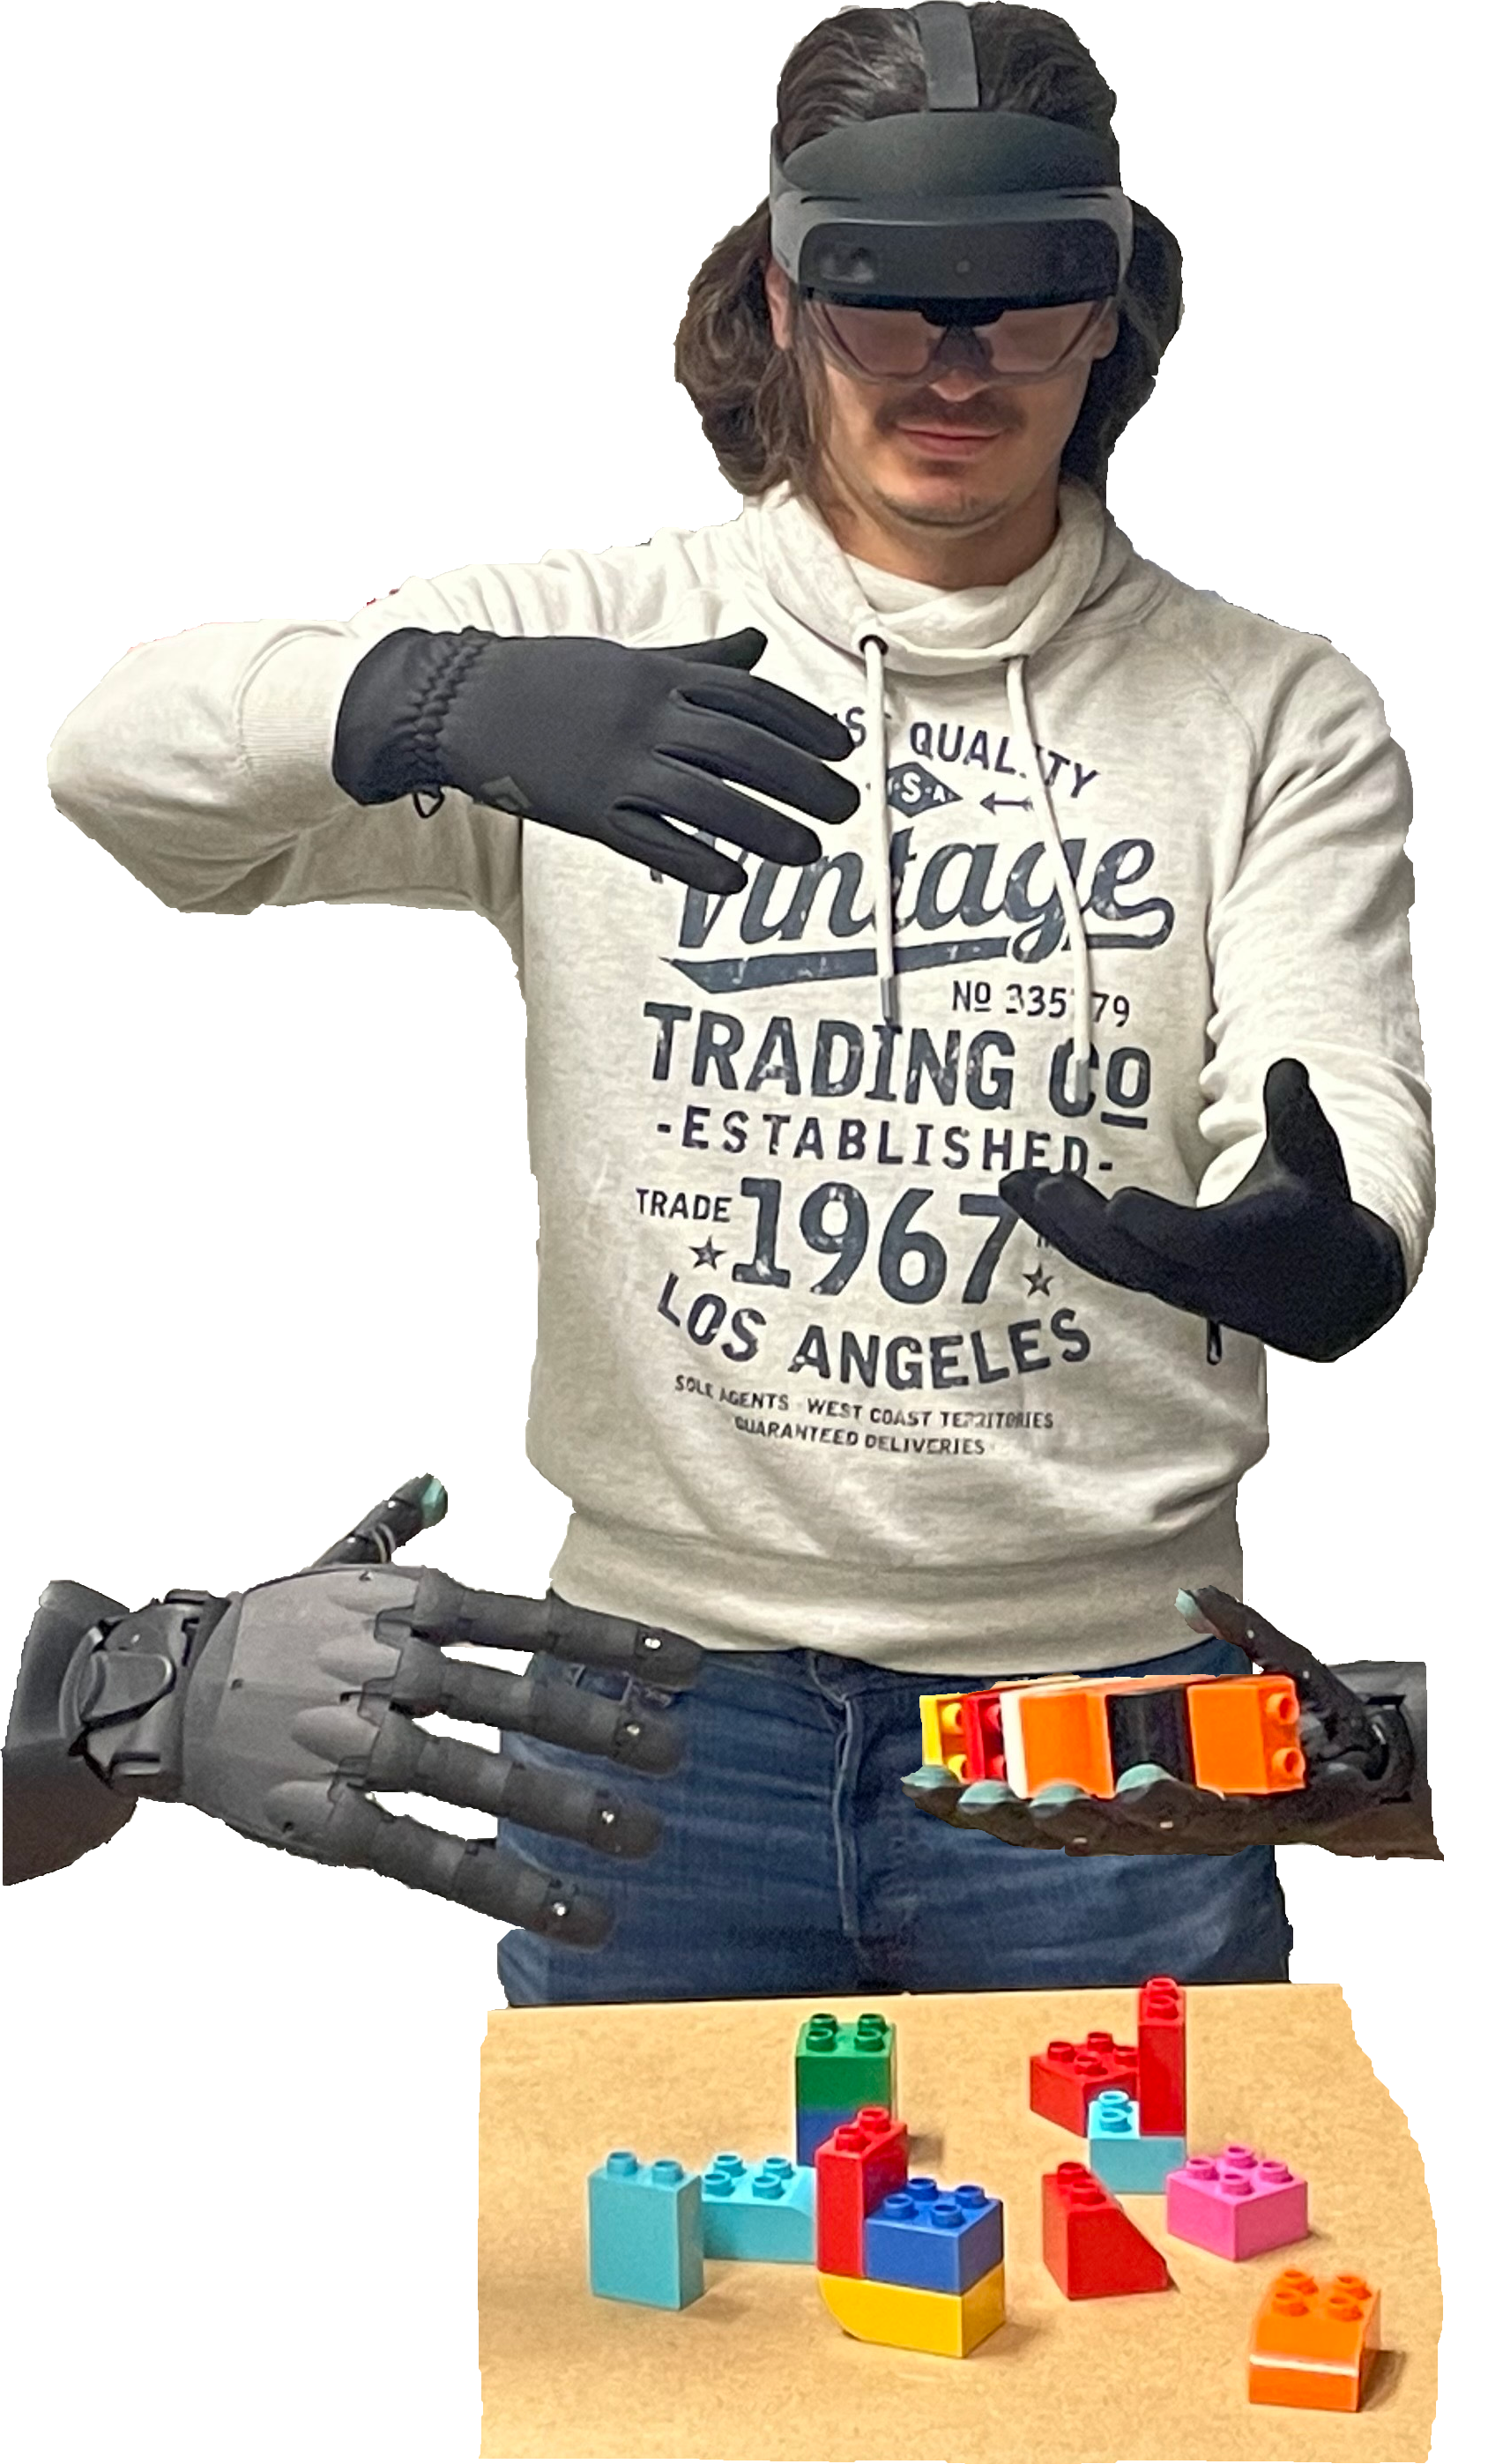
\includegraphics[width=75.56pt,height=113.63pt]{img/fig_one/human_operator.png}};
%Shape: Rectangle [id:dp9294109638439848] 
\draw  [fill={rgb, 255:red, 65; green, 117; blue, 5 }  ,fill opacity=0.5 ] (352.42,275.5) -- (475.75,275.5) -- (475.75,430) -- (352.42,430) -- cycle ;
%Shape: Rectangle [id:dp18371698149136462] 
\draw  [fill={rgb, 255:red, 255; green, 255; blue, 255 }  ,fill opacity=0.5 ][dash pattern={on 0.84pt off 2.51pt}] (360.78,301.5) -- (464.4,301.5) -- (464.4,421.5) -- (360.78,421.5) -- cycle ;
%Shape: Ellipse [id:dp956745543466187] 
\draw  [fill={rgb, 255:red, 65; green, 117; blue, 5 }  ,fill opacity=1 ] (388.83,315.9) .. controls (388.77,317.11) and (387.57,318.04) .. (386.14,317.99) .. controls (384.71,317.94) and (383.6,316.93) .. (383.66,315.72) .. controls (383.72,314.52) and (384.92,313.58) .. (386.35,313.63) .. controls (387.78,313.68) and (388.89,314.7) .. (388.83,315.9) -- cycle ;
%Shape: Ellipse [id:dp04164611278082908] 
\draw  [fill={rgb, 255:red, 65; green, 117; blue, 5 }  ,fill opacity=1 ] (388.63,309.62) .. controls (388.57,310.83) and (387.37,311.76) .. (385.94,311.71) .. controls (384.51,311.66) and (383.4,310.65) .. (383.46,309.44) .. controls (383.52,308.24) and (384.72,307.3) .. (386.15,307.35) .. controls (387.58,307.4) and (388.69,308.42) .. (388.63,309.62) -- cycle ;
%Shape: Ellipse [id:dp4061780103742162] 
\draw  [fill={rgb, 255:red, 65; green, 117; blue, 5 }  ,fill opacity=1 ] (388.9,322.38) .. controls (388.84,323.58) and (387.63,324.52) .. (386.2,324.46) .. controls (384.77,324.41) and (383.66,323.4) .. (383.72,322.19) .. controls (383.78,320.99) and (384.99,320.05) .. (386.42,320.1) .. controls (387.85,320.15) and (388.96,321.17) .. (388.9,322.38) -- cycle ;
%Shape: Ellipse [id:dp3172748756567034] 
\draw  [fill={rgb, 255:red, 65; green, 117; blue, 5 }  ,fill opacity=1 ] (388.81,329.04) .. controls (388.75,330.25) and (387.55,331.18) .. (386.12,331.13) .. controls (384.69,331.08) and (383.58,330.06) .. (383.64,328.86) .. controls (383.7,327.66) and (384.91,326.72) .. (386.34,326.77) .. controls (387.76,326.82) and (388.87,327.84) .. (388.81,329.04) -- cycle ;
%Shape: Ellipse [id:dp05860809017380075] 
\draw  [fill={rgb, 255:red, 65; green, 117; blue, 5 }  ,fill opacity=1 ] (377.6,312.9) .. controls (377.54,314.1) and (376.34,315.04) .. (374.91,314.99) .. controls (373.48,314.94) and (372.37,313.92) .. (372.43,312.72) .. controls (372.49,311.51) and (373.7,310.58) .. (375.12,310.63) .. controls (376.55,310.68) and (377.66,311.69) .. (377.6,312.9) -- cycle ;
%Shape: Ellipse [id:dp18017528139144035] 
\draw  [fill={rgb, 255:red, 65; green, 117; blue, 5 }  ,fill opacity=1 ] (377.56,319.2) .. controls (377.5,320.41) and (376.3,321.34) .. (374.87,321.29) .. controls (373.44,321.24) and (372.33,320.22) .. (372.39,319.02) .. controls (372.45,317.82) and (373.66,316.88) .. (375.08,316.93) .. controls (376.51,316.98) and (377.62,318) .. (377.56,319.2) -- cycle ;
%Shape: Ellipse [id:dp42985753660335335] 
\draw  [fill={rgb, 255:red, 65; green, 117; blue, 5 }  ,fill opacity=1 ] (377.54,325.84) .. controls (377.48,327.04) and (376.27,327.98) .. (374.85,327.93) .. controls (373.42,327.88) and (372.31,326.86) .. (372.37,325.65) .. controls (372.43,324.45) and (373.63,323.52) .. (375.06,323.57) .. controls (376.49,323.62) and (377.6,324.63) .. (377.54,325.84) -- cycle ;
%Shape: Ellipse [id:dp1969571530810924] 
\draw  [fill={rgb, 255:red, 65; green, 117; blue, 5 }  ,fill opacity=1 ] (368.58,319.2) .. controls (368.52,320.41) and (367.31,321.34) .. (365.88,321.29) .. controls (364.45,321.24) and (363.34,320.22) .. (363.4,319.02) .. controls (363.46,317.82) and (364.67,316.88) .. (366.1,316.93) .. controls (367.53,316.98) and (368.64,318) .. (368.58,319.2) -- cycle ;
%Straight Lines [id:da14310422285882574] 
\draw [fill={rgb, 255:red, 65; green, 117; blue, 5 }  ,fill opacity=1 ]   (383.64,328.86) -- (377.54,325.84) ;
%Straight Lines [id:da28848881571650553] 
\draw [fill={rgb, 255:red, 65; green, 117; blue, 5 }  ,fill opacity=1 ]   (372.39,319.02) -- (368.58,319.2) ;
%Straight Lines [id:da05563200848570238] 
\draw [fill={rgb, 255:red, 65; green, 117; blue, 5 }  ,fill opacity=1 ]   (372.37,325.65) -- (368.58,319.2) ;
%Straight Lines [id:da31451631939855085] 
\draw [fill={rgb, 255:red, 65; green, 117; blue, 5 }  ,fill opacity=1 ]   (383.46,309.44) -- (377.6,312.9) ;
%Straight Lines [id:da6357449416164839] 
\draw [fill={rgb, 255:red, 65; green, 117; blue, 5 }  ,fill opacity=1 ]   (383.46,309.44) -- (377.56,319.2) ;
%Straight Lines [id:da9280594172831405] 
\draw [fill={rgb, 255:red, 65; green, 117; blue, 5 }  ,fill opacity=1 ]   (383.46,309.44) -- (377.54,325.84) ;
%Straight Lines [id:da19935256234655652] 
\draw [fill={rgb, 255:red, 65; green, 117; blue, 5 }  ,fill opacity=1 ]   (383.66,315.72) -- (377.6,312.9) ;
%Straight Lines [id:da9870713535177682] 
\draw [fill={rgb, 255:red, 65; green, 117; blue, 5 }  ,fill opacity=1 ]   (383.66,315.72) -- (377.56,319.2) ;
%Straight Lines [id:da28358667921434233] 
\draw [fill={rgb, 255:red, 65; green, 117; blue, 5 }  ,fill opacity=1 ]   (383.66,315.72) -- (377.54,325.84) ;
%Straight Lines [id:da21288467158316915] 
\draw [fill={rgb, 255:red, 65; green, 117; blue, 5 }  ,fill opacity=1 ]   (383.72,322.19) -- (377.6,312.9) ;
%Straight Lines [id:da44685559516829054] 
\draw [fill={rgb, 255:red, 65; green, 117; blue, 5 }  ,fill opacity=1 ]   (383.72,322.19) -- (377.56,319.2) ;
%Straight Lines [id:da28998348959121556] 
\draw [fill={rgb, 255:red, 65; green, 117; blue, 5 }  ,fill opacity=1 ]   (383.72,322.19) -- (377.54,325.84) ;
%Straight Lines [id:da5161945330472014] 
\draw [fill={rgb, 255:red, 65; green, 117; blue, 5 }  ,fill opacity=1 ]   (383.64,328.86) -- (377.6,312.9) ;
%Straight Lines [id:da4249378318765743] 
\draw [fill={rgb, 255:red, 65; green, 117; blue, 5 }  ,fill opacity=1 ]   (383.64,328.86) -- (377.56,319.2) ;
%Straight Lines [id:da4917464086116057] 
\draw [fill={rgb, 255:red, 65; green, 117; blue, 5 }  ,fill opacity=1 ]   (372.43,312.72) -- (368.58,319.2) ;

%Straight Lines [id:da5549936036628806] 
\draw    (361.75,341) -- (464.25,341.5) ;
%Shape: Ellipse [id:dp9622558265336987] 
\draw  [fill={rgb, 255:red, 208; green, 2; blue, 27 }  ,fill opacity=1 ] (386.19,349.22) .. controls (386.13,350.25) and (385.05,351.06) .. (383.77,351.02) .. controls (382.48,350.97) and (381.48,350.1) .. (381.54,349.06) .. controls (381.59,348.02) and (382.68,347.22) .. (383.96,347.26) .. controls (385.24,347.3) and (386.24,348.18) .. (386.19,349.22) -- cycle ;
%Shape: Ellipse [id:dp23891232110390792] 
\draw  [fill={rgb, 255:red, 208; green, 2; blue, 27 }  ,fill opacity=1 ] (386.01,343.81) .. controls (385.95,344.84) and (384.87,345.65) .. (383.59,345.61) .. controls (382.3,345.56) and (381.3,344.69) .. (381.36,343.65) .. controls (381.41,342.61) and (382.5,341.81) .. (383.78,341.85) .. controls (385.06,341.9) and (386.06,342.77) .. (386.01,343.81) -- cycle ;
%Shape: Ellipse [id:dp3885253054881219] 
\draw  [fill={rgb, 255:red, 208; green, 2; blue, 27 }  ,fill opacity=1 ] (386.25,354.79) .. controls (386.19,355.83) and (385.11,356.63) .. (383.83,356.59) .. controls (382.54,356.55) and (381.54,355.67) .. (381.6,354.63) .. controls (381.65,353.6) and (382.74,352.79) .. (384.02,352.83) .. controls (385.3,352.88) and (386.3,353.75) .. (386.25,354.79) -- cycle ;
%Shape: Ellipse [id:dp07981508204319221] 
\draw  [fill={rgb, 255:red, 208; green, 2; blue, 27 }  ,fill opacity=1 ] (386.17,360.53) .. controls (386.12,361.57) and (385.04,362.37) .. (383.75,362.33) .. controls (382.47,362.29) and (381.47,361.41) .. (381.52,360.38) .. controls (381.58,359.34) and (382.66,358.53) .. (383.95,358.58) .. controls (385.23,358.62) and (386.23,359.5) .. (386.17,360.53) -- cycle ;
%Shape: Ellipse [id:dp17544688259790087] 
\draw  [fill={rgb, 255:red, 208; green, 2; blue, 27 }  ,fill opacity=1 ] (376.1,346.63) .. controls (376.04,347.67) and (374.96,348.47) .. (373.68,348.43) .. controls (372.39,348.38) and (371.39,347.51) .. (371.45,346.47) .. controls (371.5,345.43) and (372.59,344.63) .. (373.87,344.67) .. controls (375.15,344.72) and (376.15,345.59) .. (376.1,346.63) -- cycle ;
%Shape: Ellipse [id:dp5434200683934435] 
\draw  [fill={rgb, 255:red, 208; green, 2; blue, 27 }  ,fill opacity=1 ] (376.06,352.06) .. controls (376.01,353.09) and (374.92,353.9) .. (373.64,353.86) .. controls (372.36,353.81) and (371.36,352.94) .. (371.41,351.9) .. controls (371.47,350.86) and (372.55,350.06) .. (373.83,350.1) .. controls (375.12,350.15) and (376.12,351.02) .. (376.06,352.06) -- cycle ;
%Shape: Ellipse [id:dp23577050123729726] 
\draw  [fill={rgb, 255:red, 208; green, 2; blue, 27 }  ,fill opacity=1 ] (376.04,357.77) .. controls (375.99,358.81) and (374.9,359.61) .. (373.62,359.57) .. controls (372.34,359.53) and (371.34,358.65) .. (371.39,357.61) .. controls (371.45,356.58) and (372.53,355.77) .. (373.81,355.82) .. controls (375.1,355.86) and (376.1,356.73) .. (376.04,357.77) -- cycle ;
%Shape: Ellipse [id:dp7314567946299443] 
\draw  [fill={rgb, 255:red, 208; green, 2; blue, 27 }  ,fill opacity=1 ] (367.99,352.06) .. controls (367.93,353.09) and (366.85,353.9) .. (365.56,353.86) .. controls (364.28,353.81) and (363.28,352.94) .. (363.34,351.9) .. controls (363.39,350.86) and (364.47,350.06) .. (365.76,350.1) .. controls (367.04,350.15) and (368.04,351.02) .. (367.99,352.06) -- cycle ;
%Straight Lines [id:da1853183192523793] 
\draw [fill={rgb, 255:red, 208; green, 2; blue, 27 }  ,fill opacity=1 ]   (381.52,360.38) -- (376.04,357.77) ;
%Straight Lines [id:da7498511126808759] 
\draw [fill={rgb, 255:red, 208; green, 2; blue, 27 }  ,fill opacity=1 ]   (371.41,351.9) -- (367.98,352.06) ;
%Straight Lines [id:da32166578114627853] 
\draw [fill={rgb, 255:red, 208; green, 2; blue, 27 }  ,fill opacity=1 ]   (371.39,357.61) -- (367.98,352.06) ;
%Straight Lines [id:da6030753168944252] 
\draw [fill={rgb, 255:red, 208; green, 2; blue, 27 }  ,fill opacity=1 ]   (381.36,343.65) -- (376.1,346.63) ;
%Straight Lines [id:da3673991916183754] 
\draw [fill={rgb, 255:red, 208; green, 2; blue, 27 }  ,fill opacity=1 ]   (381.36,343.65) -- (376.06,352.06) ;
%Straight Lines [id:da06920925502035258] 
\draw [fill={rgb, 255:red, 208; green, 2; blue, 27 }  ,fill opacity=1 ]   (381.36,343.65) -- (376.04,357.77) ;
%Straight Lines [id:da41156906152273676] 
\draw [fill={rgb, 255:red, 208; green, 2; blue, 27 }  ,fill opacity=1 ]   (381.54,349.06) -- (376.1,346.63) ;
%Straight Lines [id:da11272249137571966] 
\draw [fill={rgb, 255:red, 208; green, 2; blue, 27 }  ,fill opacity=1 ]   (381.54,349.06) -- (376.06,352.06) ;
%Straight Lines [id:da21507477375332162] 
\draw [fill={rgb, 255:red, 208; green, 2; blue, 27 }  ,fill opacity=1 ]   (381.54,349.06) -- (376.04,357.77) ;
%Straight Lines [id:da36633694451164045] 
\draw [fill={rgb, 255:red, 208; green, 2; blue, 27 }  ,fill opacity=1 ]   (381.6,354.63) -- (376.1,346.63) ;
%Straight Lines [id:da1776678122843499] 
\draw [fill={rgb, 255:red, 208; green, 2; blue, 27 }  ,fill opacity=1 ]   (381.6,354.63) -- (376.06,352.06) ;
%Straight Lines [id:da9136779397639742] 
\draw [fill={rgb, 255:red, 208; green, 2; blue, 27 }  ,fill opacity=1 ]   (381.6,354.63) -- (376.04,357.77) ;
%Straight Lines [id:da3614431838017693] 
\draw [fill={rgb, 255:red, 208; green, 2; blue, 27 }  ,fill opacity=1 ]   (381.52,360.38) -- (376.1,346.63) ;
%Straight Lines [id:da27875221820730345] 
\draw [fill={rgb, 255:red, 208; green, 2; blue, 27 }  ,fill opacity=1 ]   (381.52,360.38) -- (376.06,352.06) ;
%Straight Lines [id:da23219754137091564] 
\draw [fill={rgb, 255:red, 208; green, 2; blue, 27 }  ,fill opacity=1 ]   (371.45,346.47) -- (367.98,352.06) ;

%Straight Lines [id:da7722414837186006] 
\draw    (360.75,380) -- (463.25,380.5) ;
%Shape: Axis 2D [id:dp2441388256001824] 
\draw  (366.9,406.97) -- (398.75,406.97)(370.09,387.77) -- (370.09,409.1) (391.75,401.97) -- (398.75,406.97) -- (391.75,411.97) (365.09,394.77) -- (370.09,387.77) -- (375.09,394.77)  ;
%Shape: Free Drawing [id:dp8830571424743761] 
\draw  [color={rgb, 255:red, 74; green, 144; blue, 226 }  ,draw opacity=1 ][line width=1.5] [line join = round][line cap = round] (385.42,402.6) .. controls (385.51,401.78) and (385.39,395.85) .. (387.06,395.06) .. controls (389.55,393.89) and (391.31,397.99) .. (391.77,392.77) ;
%Shape: Free Drawing [id:dp5342364622226111] 
\draw  [color={rgb, 255:red, 208; green, 2; blue, 27 }  ,draw opacity=1 ][line width=1.5] [line join = round][line cap = round] (374.92,403.1) .. controls (375.59,400.71) and (374.83,397.72) .. (375.1,395.1) .. controls (375.35,392.78) and (377.88,395.24) .. (379.04,394.1) .. controls (380.46,392.71) and (379.26,389.98) .. (378.85,388.77) ;
%Shape: Ellipse [id:dp25996553102045106] 
\draw  [fill={rgb, 255:red, 74; green, 144; blue, 226 }  ,fill opacity=1 ] (394.7,367.82) .. controls (394.65,368.73) and (393.68,369.44) .. (392.54,369.4) .. controls (391.39,369.36) and (390.5,368.59) .. (390.55,367.68) .. controls (390.6,366.77) and (391.57,366.06) .. (392.71,366.1) .. controls (393.85,366.14) and (394.74,366.91) .. (394.7,367.82) -- cycle ;
%Shape: Ellipse [id:dp12337477595337709] 
\draw  [fill={rgb, 255:red, 74; green, 144; blue, 226 }  ,fill opacity=1 ] (394.53,363.07) .. controls (394.49,363.98) and (393.52,364.69) .. (392.38,364.65) .. controls (391.23,364.61) and (390.34,363.84) .. (390.39,362.93) .. controls (390.44,362.02) and (391.41,361.31) .. (392.55,361.35) .. controls (393.69,361.39) and (394.58,362.16) .. (394.53,363.07) -- cycle ;
%Shape: Ellipse [id:dp9218205139266739] 
\draw  [fill={rgb, 255:red, 74; green, 144; blue, 226 }  ,fill opacity=1 ] (394.75,372.71) .. controls (394.7,373.62) and (393.73,374.33) .. (392.59,374.29) .. controls (391.45,374.25) and (390.56,373.48) .. (390.61,372.57) .. controls (390.65,371.66) and (391.62,370.96) .. (392.76,370.99) .. controls (393.91,371.03) and (394.8,371.8) .. (394.75,372.71) -- cycle ;
%Shape: Ellipse [id:dp42045757412856466] 
\draw  [fill={rgb, 255:red, 74; green, 144; blue, 226 }  ,fill opacity=1 ] (394.68,377.75) .. controls (394.63,378.66) and (393.67,379.37) .. (392.52,379.33) .. controls (391.38,379.29) and (390.49,378.53) .. (390.54,377.61) .. controls (390.59,376.7) and (391.55,376) .. (392.7,376.04) .. controls (393.84,376.07) and (394.73,376.84) .. (394.68,377.75) -- cycle ;
%Shape: Ellipse [id:dp43887040972020896] 
\draw  [fill={rgb, 255:red, 74; green, 144; blue, 226 }  ,fill opacity=1 ] (385.71,365.55) .. controls (385.66,366.46) and (384.69,367.16) .. (383.55,367.12) .. controls (382.4,367.09) and (381.52,366.32) .. (381.56,365.41) .. controls (381.61,364.5) and (382.58,363.79) .. (383.72,363.83) .. controls (384.86,363.87) and (385.75,364.63) .. (385.71,365.55) -- cycle ;
%Shape: Ellipse [id:dp8505831460928501] 
\draw  [fill={rgb, 255:red, 74; green, 144; blue, 226 }  ,fill opacity=1 ] (385.67,370.31) .. controls (385.63,371.22) and (384.66,371.93) .. (383.52,371.89) .. controls (382.37,371.85) and (381.48,371.08) .. (381.53,370.17) .. controls (381.58,369.26) and (382.54,368.56) .. (383.69,368.59) .. controls (384.83,368.63) and (385.72,369.4) .. (385.67,370.31) -- cycle ;
%Shape: Ellipse [id:dp5048676158581518] 
\draw  [fill={rgb, 255:red, 74; green, 144; blue, 226 }  ,fill opacity=1 ] (385.66,375.33) .. controls (385.61,376.24) and (384.64,376.95) .. (383.5,376.91) .. controls (382.35,376.87) and (381.46,376.1) .. (381.51,375.19) .. controls (381.56,374.28) and (382.53,373.57) .. (383.67,373.61) .. controls (384.81,373.65) and (385.7,374.42) .. (385.66,375.33) -- cycle ;
%Shape: Ellipse [id:dp05662114592079792] 
\draw  [fill={rgb, 255:red, 74; green, 144; blue, 226 }  ,fill opacity=1 ] (378.48,370.31) .. controls (378.43,371.22) and (377.46,371.93) .. (376.32,371.89) .. controls (375.18,371.85) and (374.29,371.08) .. (374.34,370.17) .. controls (374.38,369.26) and (375.35,368.56) .. (376.49,368.59) .. controls (377.64,368.63) and (378.53,369.4) .. (378.48,370.31) -- cycle ;
%Straight Lines [id:da15120101419612508] 
\draw [fill={rgb, 255:red, 74; green, 144; blue, 226 }  ,fill opacity=1 ]   (390.54,377.61) -- (385.65,375.33) ;
%Straight Lines [id:da6781524910980562] 
\draw [fill={rgb, 255:red, 74; green, 144; blue, 226 }  ,fill opacity=1 ]   (381.53,370.17) -- (378.48,370.31) ;
%Straight Lines [id:da6071953381520283] 
\draw [fill={rgb, 255:red, 74; green, 144; blue, 226 }  ,fill opacity=1 ]   (381.51,375.19) -- (378.48,370.31) ;
%Straight Lines [id:da5380240008552817] 
\draw [fill={rgb, 255:red, 74; green, 144; blue, 226 }  ,fill opacity=1 ]   (390.39,362.93) -- (385.71,365.55) ;
%Straight Lines [id:da1945824448733846] 
\draw [fill={rgb, 255:red, 74; green, 144; blue, 226 }  ,fill opacity=1 ]   (390.39,362.93) -- (385.67,370.31) ;
%Straight Lines [id:da09422142537560174] 
\draw [fill={rgb, 255:red, 74; green, 144; blue, 226 }  ,fill opacity=1 ]   (390.39,362.93) -- (385.65,375.33) ;
%Straight Lines [id:da7910388453331011] 
\draw [fill={rgb, 255:red, 74; green, 144; blue, 226 }  ,fill opacity=1 ]   (390.55,367.68) -- (385.71,365.55) ;
%Straight Lines [id:da8072770269531041] 
\draw [fill={rgb, 255:red, 74; green, 144; blue, 226 }  ,fill opacity=1 ]   (390.55,367.68) -- (385.67,370.31) ;
%Straight Lines [id:da8358999097052429] 
\draw [fill={rgb, 255:red, 74; green, 144; blue, 226 }  ,fill opacity=1 ]   (390.55,367.68) -- (385.65,375.33) ;
%Straight Lines [id:da06406375572669465] 
\draw [fill={rgb, 255:red, 74; green, 144; blue, 226 }  ,fill opacity=1 ]   (390.61,372.57) -- (385.71,365.55) ;
%Straight Lines [id:da9204679674221412] 
\draw [fill={rgb, 255:red, 74; green, 144; blue, 226 }  ,fill opacity=1 ]   (390.61,372.57) -- (385.67,370.31) ;
%Straight Lines [id:da1499502487264115] 
\draw [fill={rgb, 255:red, 74; green, 144; blue, 226 }  ,fill opacity=1 ]   (390.61,372.57) -- (385.65,375.33) ;
%Straight Lines [id:da026037684396199468] 
\draw [fill={rgb, 255:red, 74; green, 144; blue, 226 }  ,fill opacity=1 ]   (390.54,377.61) -- (385.71,365.55) ;
%Straight Lines [id:da06751377716998264] 
\draw [fill={rgb, 255:red, 74; green, 144; blue, 226 }  ,fill opacity=1 ]   (390.54,377.61) -- (385.67,370.31) ;
%Straight Lines [id:da9797857571778305] 
\draw [fill={rgb, 255:red, 74; green, 144; blue, 226 }  ,fill opacity=1 ]   (381.56,365.41) -- (378.48,370.31) ;

%Straight Lines [id:da060525167879017405] 
\draw [line width=1.5]    (230.33,88) -- (244,88.26) ;
\draw [shift={(248,88.33)}, rotate = 181.08] [fill={rgb, 255:red, 0; green, 0; blue, 0 }  ][line width=0.08]  [draw opacity=0] (9.29,-4.46) -- (0,0) -- (9.29,4.46) -- cycle    ;
%Image [id:dp3810151117321877] 
\draw (132.35,316.13) node  {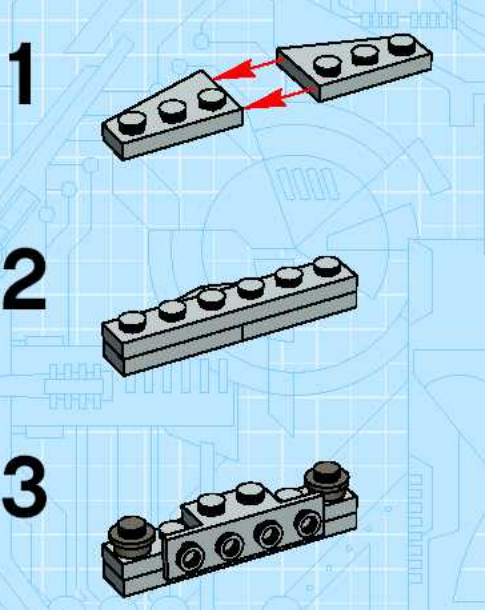
\includegraphics[width=34.73pt,height=52.5pt]{img/fig_one/lego_orig_manuals1.png}};
%Image [id:dp2488978448835365] 
\draw (132.1,386.13) node  {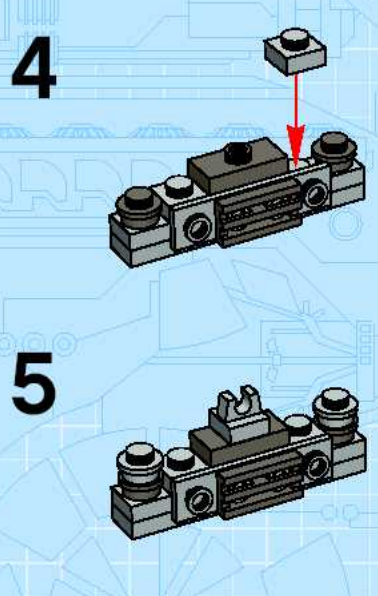
\includegraphics[width=34.35pt,height=52.5pt]{img/fig_one/lego_orig_manuals2.png}};
%Image [id:dp8581971273563807] 
\draw (551.08,65.83) node  {
\includegraphics[width=20.88pt,height=19.25pt]{img/fig_one/pairwise_comparissons.png}};
%Image [id:dp6865157205733583] 
\draw (613.42,66.17) node  {
\includegraphics[width=17.88pt,height=16.25pt]{img/fig_one/corrections.png}};
%Straight Lines [id:da9074013588403695] 
\draw [line width=0.75]    (370.3,110.2) -- (639,110.33) ;

% Text Node
\draw  [fill={rgb, 255:red, 14; green, 1; blue, 1 }  ,fill opacity=0.2 ][dash pattern={on 0.84pt off 2.51pt}]  (370.6,76.92) -- (431.6,76.92) -- (431.6,109.92) -- (370.6,109.92) -- cycle  ;
\draw (366.6,80.92) node [anchor=north west][inner sep=0.75pt]  [font=\scriptsize] [align=left] {\begin{minipage}[lt]{50.42pt}\setlength\topsep{0pt}
\begin{center}
{\fontfamily{ptm}\selectfont Demonstra-}\\{\fontfamily{ptm}\selectfont tions}
\end{center}

\end{minipage}};
% Text Node
\draw  [color={rgb, 255:red, 65; green, 117; blue, 5 }  ,draw opacity=1 ][fill={rgb, 255:red, 65; green, 117; blue, 5 }  ,fill opacity=0.2 ][dash pattern={on 0.84pt off 2.51pt}]  (39,42) -- (133,42) -- (133,61) -- (39,61) -- cycle  ;
\draw (42,46) node [anchor=north west][inner sep=0.75pt]  [font=\scriptsize] [align=left] {{\fontfamily{ptm}\selectfont Planned Trajectories}};
% Text Node
\draw  [color={rgb, 255:red, 74; green, 144; blue, 226 }  ,draw opacity=1 ][fill={rgb, 255:red, 74; green, 144; blue, 226 }  ,fill opacity=0.2 ][dash pattern={on 0.84pt off 2.51pt}]  (72.2,65.2) -- (167.2,65.2) -- (167.2,84.2) -- (72.2,84.2) -- cycle  ;
\draw (75.2,69.2) node [anchor=north west][inner sep=0.75pt]  [font=\scriptsize] [align=left] {{\fontfamily{ptm}\selectfont Scene Visualizations}};
% Text Node
\draw  [color={rgb, 255:red, 144; green, 19; blue, 254 }  ,draw opacity=1 ][fill={rgb, 255:red, 144; green, 19; blue, 254 }  ,fill opacity=0.2 ][dash pattern={on 0.84pt off 2.51pt}]  (99.2,88.2) -- (182.2,88.2) -- (182.2,107.2) -- (99.2,107.2) -- cycle  ;
\draw (102.2,92.2) node [anchor=north west][inner sep=0.75pt]  [font=\scriptsize] [align=left] {{\fontfamily{ptm}\selectfont Scene Predictions}};
% Text Node
\draw (164.73,191.1) node [anchor=north west][inner sep=0.75pt]  [font=\normalsize,color={rgb, 255:red, 0; green, 0; blue, 0 }  ,opacity=1 ] [align=left] {\begin{minipage}[lt]{48.94pt}\setlength\topsep{0pt}
{\fontfamily{ptm}\selectfont \textbf{Continual }}
\begin{center}
{\fontfamily{ptm}\selectfont \textbf{Learning}}
\end{center}

\end{minipage}};
% Text Node
\draw  [color={rgb, 255:red, 208; green, 2; blue, 27 }  ,draw opacity=1 ][fill={rgb, 255:red, 208; green, 2; blue, 27 }  ,fill opacity=0.2 ][dash pattern={on 0.84pt off 2.51pt}]  (125.45,114.95) -- (195.45,114.95) -- (195.45,147.95) -- (125.45,147.95) -- cycle  ;
\draw (128.45,118.95) node [anchor=north west][inner sep=0.75pt]  [font=\scriptsize] [align=left] {Manipulation \\Assessments};
% Text Node
\draw (505.07,332.25) node [anchor=north west][inner sep=0.75pt]   [align=left] {Simulation};
% Text Node
\draw (504.4,405.92) node [anchor=north west][inner sep=0.75pt]   [align=left] {{\fontfamily{ptm}\selectfont Real World}};
% Text Node
\draw (250.4,301.08) node [anchor=north west][inner sep=0.75pt]  [font=\normalsize] [align=left] {{\fontfamily{ptm}\selectfont Perception }};
% Text Node
\draw (297.5,252) node [anchor=north west][inner sep=0.75pt]   [align=left] {{\fontfamily{ptm}\selectfont Foundation Models}};
% Text Node
\draw (41.42,164.9) node [anchor=north west][inner sep=0.75pt]   [align=left] {\begin{minipage}[lt]{62.76pt}\setlength\topsep{0pt}
\begin{center}
{\fontfamily{ptm}\selectfont Robot's Task }\\{\fontfamily{ptm}\selectfont Understanding}
\end{center}

\end{minipage}};
% Text Node
\draw (440.17,37.57) node [anchor=north west][inner sep=0.75pt]   [align=left] {{\fontfamily{ptm}\selectfont Human Feedback}};
% Text Node
\draw (258.43,414.18) node [anchor=north west][inner sep=0.75pt]  [font=\normalsize] [align=left] { Reward };
% Text Node
\draw (253.53,356.25) node [anchor=north west][inner sep=0.75pt]  [font=\normalsize] [align=left] {Dynamics};
% Text Node
\draw (250.63,21.75) node [anchor=north west][inner sep=0.75pt]   [align=left] {{\fontfamily{ptm}\selectfont Human Operator}};
% Text Node
\draw  [line width=2.25]   (204.5,22.5) -- (229.5,22.5) -- (229.5,175.5) -- (204.5,175.5) -- cycle  ;
\draw (223.5,25.5) node [anchor=north west][inner sep=0.75pt]  [rotate=-90] [align=left] {{\fontfamily{ptm}\selectfont AR-Based Visualization}};
% Text Node
\draw (558.03,160.97) node [anchor=north west][inner sep=0.75pt]   [align=left] {\begin{minipage}[lt]{52.51pt}\setlength\topsep{0pt}
\begin{center}
{\fontfamily{ptm}\selectfont Bayesian}
\end{center}
{\fontfamily{ptm}\selectfont Fine Tuning}
\end{minipage}};
% Text Node
\draw (473.22,162.05) node [anchor=north west][inner sep=0.75pt]   [align=left] {\begin{minipage}[lt]{39.53pt}\setlength\topsep{0pt}
\begin{center}
{\fontfamily{ptm}\selectfont Meta }\\{\fontfamily{ptm}\selectfont Learning}
\end{center}

\end{minipage}};
% Text Node
\draw (373.7,162.3) node [anchor=north west][inner sep=0.75pt]   [align=left] {\begin{minipage}[lt]{48.86pt}\setlength\topsep{0pt}
\begin{center}
{\fontfamily{ptm}\selectfont Interactive }\\{\fontfamily{ptm}\selectfont RL}
\end{center}

\end{minipage}};
% Text Node
\draw (390.04,312.53) node [anchor=north west][inner sep=0.75pt]   [align=left] {{\fontfamily{ptm}\selectfont High-Level }};
% Text Node
\draw (394,350.5) node [anchor=north west][inner sep=0.75pt]   [align=left] {{\fontfamily{ptm}\selectfont Low-Level }};
% Text Node
\draw (357,282.5) node [anchor=north west][inner sep=0.75pt]   [align=left] {Hierarchical Skill};
% Text Node
\draw (403,385) node [anchor=north west][inner sep=0.75pt]   [align=left] {{\fontfamily{ptm}\selectfont Motion }\\{\fontfamily{ptm}\selectfont Primitive}};
% Text Node
\draw (105.38,424.76) node [anchor=north west][inner sep=0.75pt]   [align=left] {{\fontfamily{ptm}\selectfont Manuals}};
% Text Node
\draw  [fill={rgb, 255:red, 14; green, 1; blue, 1 }  ,fill opacity=0.2 ][dash pattern={on 0.84pt off 2.51pt}]  (593.93,76.92) -- (634.93,76.92) -- (634.93,109.92) -- (593.93,109.92) -- cycle  ;
\draw (596.93,80.92) node [anchor=north west][inner sep=0.75pt]  [font=\scriptsize] [align=left] {\begin{minipage}[lt]{25.33pt}\setlength\topsep{0pt}
\begin{center}
{\fontfamily{ptm}\selectfont Correc-}\\{\fontfamily{ptm}\selectfont tions}
\end{center}

\end{minipage}};
% Text Node
\draw  [fill={rgb, 255:red, 14; green, 1; blue, 1 }  ,fill opacity=0.2 ][dash pattern={on 0.84pt off 2.51pt}]  (518.6,76.92) -- (581.6,76.92) -- (581.6,109.92) -- (518.6,109.92) -- cycle  ;
\draw (521.6,80.92) node [anchor=north west][inner sep=0.75pt]  [font=\scriptsize] [align=left] {\begin{minipage}[lt]{40.4pt}\setlength\topsep{0pt}
\begin{center}
{\fontfamily{ptm}\selectfont Pairwise }\\{\fontfamily{ptm}\selectfont Comparisons}
\end{center}

\end{minipage}};
% Text Node
\draw  [fill={rgb, 255:red, 14; green, 1; blue, 1 }  ,fill opacity=0.2 ][dash pattern={on 0.84pt off 2.51pt}]  (445.6,76.92) -- (503.6,76.92) -- (503.6,109.92) -- (445.6,109.92) -- cycle  ;
\draw (448.6,80.92) node [anchor=north west][inner sep=0.75pt]  [font=\scriptsize] [align=left] {\begin{minipage}[lt]{36.44pt}\setlength\topsep{0pt}
\begin{center}
{\fontfamily{ptm}\selectfont Verbal }\\{\fontfamily{ptm}\selectfont Instructions}
\end{center}

\end{minipage}};


\end{tikzpicture}
